%%%%%%%%%%%%%%%%%%%%%%%%%%%%%%%%%%%%%%%%%%%%%%%%%%%%%%%%%%%%%%%%%%%%%%%%%%%%%%%%%%%%%%%%%%%%%%%%%%%%%%%%%%%%%%%%%%%%%%%%%%%%%%%%%%%%%%%%%%%%%%%%%%%%%%%%%%%%%%%%%%%
% Written By Michael Brodskiy
% Class: Fundamentals of Electronics
% Professor: M. Onabajo
%%%%%%%%%%%%%%%%%%%%%%%%%%%%%%%%%%%%%%%%%%%%%%%%%%%%%%%%%%%%%%%%%%%%%%%%%%%%%%%%%%%%%%%%%%%%%%%%%%%%%%%%%%%%%%%%%%%%%%%%%%%%%%%%%%%%%%%%%%%%%%%%%%%%%%%%%%%%%%%%%%%

\include{Includes.tex}

\title{Homework 12}
\date{\today}
\author{Michael Brodskiy\\ \small Professor: M. Onabajo}

\begin{document}

\maketitle

\begin{enumerate}

  \item

    \begin{enumerate}

      \item $D=ABC+\overline{AB}$

        We begin by constructing the table. First, we put in each combination of inputs. Given that there are 3 inputs, there should be $2^3=8$ combinations:

        \begin{center}
          \begin{tabular}[H]{|c|c|c|c|}
            \hline
            A & B & C & D\\
            \hline
            0 & 0 & 0 & 0\\
            \hline
            0 & 0 & 1 & 0\\
            \hline
            0 & 1 & 0 & 0\\
            \hline
            1 & 0 & 0 & 1\\
            \hline
            0 & 1 & 1 & 0\\
            \hline
            1 & 0 & 1 & 1\\
            \hline
            1 & 1 & 0 & 0\\
            \hline
            1 & 1 & 1 & 1\\
            \hline
          \end{tabular}
        \end{center}

        From here, we can draw the circuit as:

        \begin{figure}[H]
          \centering
          \tikzset{every picture/.style={line width=0.75pt}} %set default line width to 0.75pt        

\begin{tikzpicture}[x=0.75pt,y=0.75pt,yscale=-1,xscale=1]
%uncomment if require: \path (0,393); %set diagram left start at 0, and has height of 393

%Straight Lines [id:da23815456210484298] 
\draw    (131.71,157) -- (81.64,157) ;
\draw [shift={(79.29,157)}, rotate = 180] [color={rgb, 255:red, 0; green, 0; blue, 0 }  ][line width=0.75]      (0, 0) circle [x radius= 3.35, y radius= 3.35]   ;
%Straight Lines [id:da04610179645106571] 
\draw    (131.71,189) -- (81.64,189) ;
\draw [shift={(79.29,189)}, rotate = 180] [color={rgb, 255:red, 0; green, 0; blue, 0 }  ][line width=0.75]      (0, 0) circle [x radius= 3.35, y radius= 3.35]   ;
%Straight Lines [id:da7638407091081825] 
\draw    (131.71,221) -- (81.64,221) ;
\draw [shift={(79.29,221)}, rotate = 180] [color={rgb, 255:red, 0; green, 0; blue, 0 }  ][line width=0.75]      (0, 0) circle [x radius= 3.35, y radius= 3.35]   ;
%Shape: And Gate [id:dp1564557077664277] 
\draw   (147.71,149) -- (171.71,149) .. controls (184.96,149) and (195.71,159.75) .. (195.71,173) .. controls (195.71,186.25) and (184.96,197) .. (171.71,197) -- (147.71,197) -- (147.71,149) -- cycle (131.71,157) -- (147.71,157) (131.71,189) -- (147.71,189) (195.71,173) -- (211.71,173) ;
%Shape: And Gate [id:dp07355261068451113] 
\draw   (246.13,165) -- (270.13,165) .. controls (283.38,165) and (294.13,175.75) .. (294.13,189) .. controls (294.13,202.25) and (283.38,213) .. (270.13,213) -- (246.13,213) -- (246.13,165) -- cycle (230.13,173) -- (246.13,173) (230.13,205) -- (246.13,205) (294.13,189) -- (310.13,189) ;
%Straight Lines [id:da4661863224212748] 
\draw    (230.13,173) -- (211.71,173) ;
%Straight Lines [id:da3821485817926048] 
\draw    (230.13,205) -- (131.71,205) ;
%Straight Lines [id:da9213385284221522] 
\draw    (131.71,221) -- (131.71,205) ;
%Straight Lines [id:da9899457357378714] 
\draw    (408.55,189) -- (310.13,189) ;
%Straight Lines [id:da2621263792990446] 
\draw    (408.13,79) -- (408.55,157) ;
%Straight Lines [id:da026515041729731847] 
\draw    (488.55,173) -- (538.62,173) ;
\draw [shift={(540.97,173)}, rotate = 0] [color={rgb, 255:red, 0; green, 0; blue, 0 }  ][line width=0.75]      (0, 0) circle [x radius= 3.35, y radius= 3.35]   ;
%Straight Lines [id:da3970001006084427] 
\draw    (220,78.29) -- (220,172.71) ;
%Shape: Not/Inverter Gate [id:dp48812914811132324] 
\draw   (234.81,48.29) -- (279.26,78.29) -- (234.81,108.29) -- (234.81,48.29) -- cycle (220,78.29) -- (234.81,78.29) (288.15,78.29) -- (300,78.29) (279.26,78.29) .. controls (279.26,74.98) and (281.25,72.29) .. (283.7,72.29) .. controls (286.16,72.29) and (288.15,74.98) .. (288.15,78.29) .. controls (288.15,81.6) and (286.16,84.29) .. (283.7,84.29) .. controls (281.25,84.29) and (279.26,81.6) .. (279.26,78.29) -- cycle ;
%Straight Lines [id:da25799347375209314] 
\draw    (408.13,79) -- (300,78.29) ;
%Shape: Or Gate [id:dp8158339008286285] 
\draw   (420.55,148.58) -- (440.55,148.58) .. controls (454.51,149.02) and (466.98,158.47) .. (472.55,172.83) .. controls (466.98,187.2) and (454.51,196.65) .. (440.55,197.08) -- (420.55,197.08) .. controls (429.13,182.08) and (429.13,163.59) .. (420.55,148.58) -- cycle (408.55,156.67) -- (424.55,156.67) (408.55,189) -- (424.55,189) (472.55,172.83) -- (488.55,172.83) ;

% Text Node
\draw (79.29,150.6) node [anchor=south] [inner sep=0.75pt]    {$A$};
% Text Node
\draw (79.29,182.6) node [anchor=south] [inner sep=0.75pt]    {$B$};
% Text Node
\draw (79.29,214.6) node [anchor=south] [inner sep=0.75pt]    {$C$};
% Text Node
\draw (220,176.11) node [anchor=north] [inner sep=0.75pt]    {$AB$};
% Text Node
\draw (314.13,185.6) node [anchor=south] [inner sep=0.75pt]    {$ABC$};
% Text Node
\draw (540.97,166.6) node [anchor=south] [inner sep=0.75pt]    {$D=ABC+\overline{AB}$};
% Text Node
\draw (354.07,75.24) node [anchor=south] [inner sep=0.75pt]    {$\overline{AB}$};


\end{tikzpicture}

          \caption{Logic Circuit for 1a}
          \label{fig:1}
        \end{figure}

      \item $E=AB+A\overline{B}C+\overline{C}D$

        Once again, we begin by analyzing each combination. Since there are 4 inputs, there are $2^4=16$ possible inputs. This gives us:

        \begin{center}
          \begin{tabular}[H]{|c|c|c|c|c|}
            \hline
            A & B & C & D & E\\
            \hline
            0 & 0 & 0 & 0 & 0\\
            \hline
            0 & 0 & 0 & 1 & 1\\
            \hline
            0 & 0 & 1 & 0 & 0\\
            \hline
            0 & 1 & 0 & 0 & 0\\
            \hline
            1 & 0 & 0 & 0 & 0\\
            \hline
            0 & 0 & 1 & 1 & 0\\
            \hline
            0 & 1 & 0 & 1 & 1\\
            \hline
            1 & 0 & 0 & 1 & 1\\
            \hline
            0 & 1 & 1 & 0 & 0\\
            \hline
            1 & 0 & 1 & 0 & 1\\
            \hline
            1 & 1 & 0 & 0 & 1\\
            \hline
            0 & 1 & 1 & 1 & 0\\
            \hline
            1 & 0 & 1 & 1 & 1\\
            \hline
            1 & 1 & 1 & 0 & 1\\
            \hline
            1 & 1 & 0 & 1 & 1\\
            \hline
            1 & 1 & 1 & 1 & 1\\
            \hline
          \end{tabular}
        \end{center}

        This gives us the following circuit:

        \begin{figure}[H]
          \centering
          \tikzset{every picture/.style={line width=0.75pt}} %set default line width to 0.75pt        

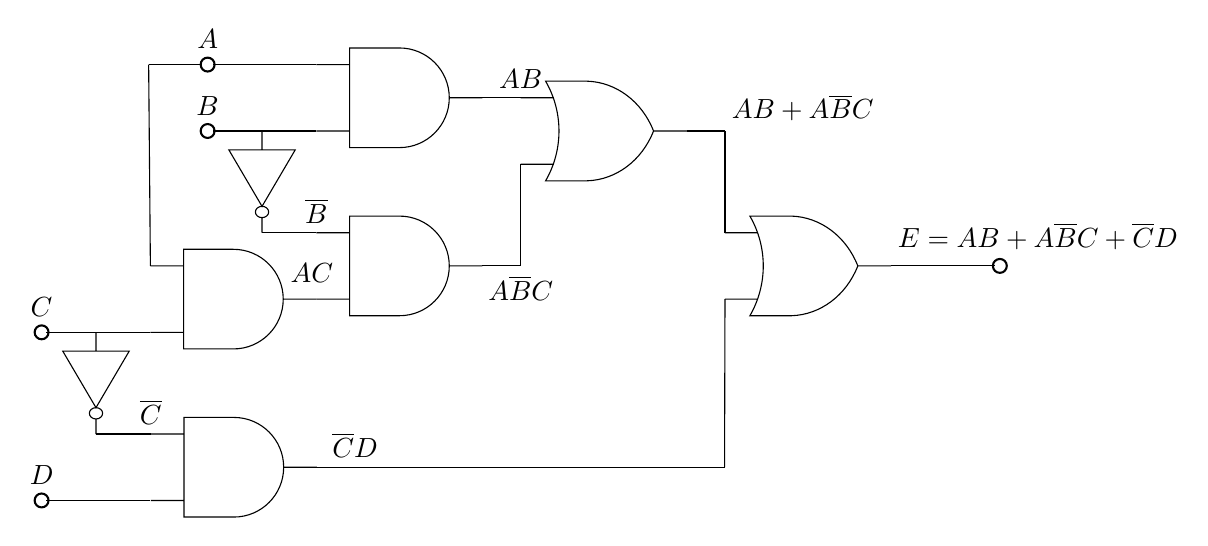
\begin{tikzpicture}[x=0.75pt,y=0.75pt,yscale=-1,xscale=1]
%uncomment if require: \path (0,393); %set diagram left start at 0, and has height of 393

%Straight Lines [id:da23815456210484298] 
\draw    (189.71,157) -- (139.64,157) ;
\draw [shift={(137.29,157)}, rotate = 180] [color={rgb, 255:red, 0; green, 0; blue, 0 }  ][line width=0.75]      (0, 0) circle [x radius= 3.35, y radius= 3.35]   ;
%Straight Lines [id:da04610179645106571] 
\draw    (189.71,189) -- (139.64,189) ;
\draw [shift={(137.29,189)}, rotate = 180] [color={rgb, 255:red, 0; green, 0; blue, 0 }  ][line width=0.75]      (0, 0) circle [x radius= 3.35, y radius= 3.35]   ;
%Straight Lines [id:da7638407091081825] 
\draw    (109.71,286) -- (59.64,286) ;
\draw [shift={(57.29,286)}, rotate = 180] [color={rgb, 255:red, 0; green, 0; blue, 0 }  ][line width=0.75]      (0, 0) circle [x radius= 3.35, y radius= 3.35]   ;
%Shape: And Gate [id:dp1564557077664277] 
\draw   (205.71,149) -- (229.71,149) .. controls (242.96,149) and (253.71,159.75) .. (253.71,173) .. controls (253.71,186.25) and (242.96,197) .. (229.71,197) -- (205.71,197) -- (205.71,149) -- cycle (189.71,157) -- (205.71,157) (189.71,189) -- (205.71,189) (253.71,173) -- (269.71,173) ;
%Straight Lines [id:da4661863224212748] 
\draw    (288.13,173) -- (269.71,173) ;
%Straight Lines [id:da3326289809840617] 
\draw    (109.71,367) -- (59.64,367) ;
\draw [shift={(57.29,367)}, rotate = 180] [color={rgb, 255:red, 0; green, 0; blue, 0 }  ][line width=0.75]      (0, 0) circle [x radius= 3.35, y radius= 3.35]   ;
%Shape: And Gate [id:dp7425325553134294] 
\draw   (205.71,230) -- (229.71,230) .. controls (242.96,230) and (253.71,240.75) .. (253.71,254) .. controls (253.71,267.25) and (242.96,278) .. (229.71,278) -- (205.71,278) -- (205.71,230) -- cycle (189.71,238) -- (205.71,238) (189.71,270) -- (205.71,270) (253.71,254) -- (269.71,254) ;
%Shape: Not/Inverter Gate [id:dp730124212850165] 
\draw   (179.5,198.07) -- (163.5,225.3) -- (147.5,198.07) -- (179.5,198.07) -- cycle (163.5,189) -- (163.5,198.07) (163.5,230.74) -- (163.5,238) (163.5,225.3) .. controls (165.27,225.3) and (166.7,226.52) .. (166.7,228.02) .. controls (166.7,229.52) and (165.27,230.74) .. (163.5,230.74) .. controls (161.73,230.74) and (160.3,229.52) .. (160.3,228.02) .. controls (160.3,226.52) and (161.73,225.3) .. (163.5,225.3) -- cycle ;
%Straight Lines [id:da4080679153459019] 
\draw    (189.71,238) -- (163.29,238) ;
%Straight Lines [id:da606928960379901] 
\draw    (288.13,254) -- (269.71,254) ;
%Shape: And Gate [id:dp3055341920246588] 
\draw   (125.71,246) -- (149.71,246) .. controls (162.96,246) and (173.71,256.75) .. (173.71,270) .. controls (173.71,283.25) and (162.96,294) .. (149.71,294) -- (125.71,294) -- (125.71,246) -- cycle (109.71,254) -- (125.71,254) (109.71,286) -- (125.71,286) (173.71,270) -- (189.71,270) ;
%Straight Lines [id:da26894829773415774] 
\draw    (108.87,157) -- (109.71,254) ;
%Straight Lines [id:da8173885985145962] 
\draw    (134.29,157) -- (108.87,157) ;
%Shape: Not/Inverter Gate [id:dp40034937466347376] 
\draw   (99.5,295.07) -- (83.5,322.3) -- (67.5,295.07) -- (99.5,295.07) -- cycle (83.5,286) -- (83.5,295.07) (83.5,327.74) -- (83.5,335) (83.5,322.3) .. controls (85.27,322.3) and (86.7,323.52) .. (86.7,325.02) .. controls (86.7,326.52) and (85.27,327.74) .. (83.5,327.74) .. controls (81.73,327.74) and (80.3,326.52) .. (80.3,325.02) .. controls (80.3,323.52) and (81.73,322.3) .. (83.5,322.3) -- cycle ;
%Straight Lines [id:da9187250725995942] 
\draw    (109.92,335) -- (83.5,335) ;
%Shape: And Gate [id:dp5737189415520882] 
\draw   (125.92,327) -- (149.92,327) .. controls (163.17,327) and (173.92,337.75) .. (173.92,351) .. controls (173.92,364.25) and (163.17,375) .. (149.92,375) -- (125.92,375) -- (125.92,327) -- cycle (109.92,335) -- (125.92,335) (109.92,367) -- (125.92,367) (173.92,351) -- (189.92,351) ;
%Straight Lines [id:da9286960259513112] 
\draw    (208.34,351) -- (189.92,351) ;
%Shape: Or Gate [id:dp8962192080668689] 
\draw   (300.13,165) -- (320.13,165) .. controls (334.08,165.43) and (346.55,174.78) .. (352.13,189) .. controls (346.55,203.22) and (334.08,212.57) .. (320.13,213) -- (300.13,213) .. controls (308.71,198.15) and (308.71,179.85) .. (300.13,165) -- cycle (288.13,173) -- (304.13,173) (288.13,205) -- (304.13,205) (352.13,189) -- (368.13,189) ;
%Straight Lines [id:da47934517298171864] 
\draw    (288.13,205) -- (288.13,254) ;
%Straight Lines [id:da5106515434171844] 
\draw    (386.55,189) -- (368.13,189) ;
%Shape: Or Gate [id:dp5422231005469561] 
\draw   (398.55,230) -- (418.55,230) .. controls (432.51,230.43) and (444.98,239.78) .. (450.55,254) .. controls (444.98,268.22) and (432.51,277.57) .. (418.55,278) -- (398.55,278) .. controls (407.13,263.15) and (407.13,244.85) .. (398.55,230) -- cycle (386.55,238) -- (402.55,238) (386.55,270) -- (402.55,270) (450.55,254) -- (466.55,254) ;
%Straight Lines [id:da07386764887877606] 
\draw    (386.55,189) -- (386.55,238) ;
%Straight Lines [id:da919048777312122] 
\draw    (386.55,270) -- (386.34,351) ;
%Straight Lines [id:da07474028966591151] 
\draw    (386.34,351) -- (208.34,351) ;
%Straight Lines [id:da6374195858525608] 
\draw    (466.55,254) -- (516.62,254) ;
\draw [shift={(518.97,254)}, rotate = 0] [color={rgb, 255:red, 0; green, 0; blue, 0 }  ][line width=0.75]      (0, 0) circle [x radius= 3.35, y radius= 3.35]   ;

% Text Node
\draw (137.29,150.6) node [anchor=south] [inner sep=0.75pt]    {$A$};
% Text Node
\draw (137.29,182.6) node [anchor=south] [inner sep=0.75pt]    {$B$};
% Text Node
\draw (57.29,279.6) node [anchor=south] [inner sep=0.75pt]    {$C$};
% Text Node
\draw (288.13,169.6) node [anchor=south] [inner sep=0.75pt]    {$AB$};
% Text Node
\draw (57.29,360.6) node [anchor=south] [inner sep=0.75pt]    {$D$};
% Text Node
\draw (189.71,234.6) node [anchor=south] [inner sep=0.75pt]    {$\overline{B}$};
% Text Node
\draw (288.13,257.4) node [anchor=north] [inner sep=0.75pt]    {$A\overline{B} C$};
% Text Node
\draw (176,251.4) node [anchor=north west][inner sep=0.75pt]    {$AC$};
% Text Node
\draw (208.34,347.6) node [anchor=south] [inner sep=0.75pt]    {$\overline{C} D$};
% Text Node
\draw (109.92,331.6) node [anchor=south] [inner sep=0.75pt]    {$\overline{C}$};
% Text Node
\draw (388.55,185.6) node [anchor=south west] [inner sep=0.75pt]    {$AB+A\overline{B} C$};
% Text Node
\draw (468.55,247.6) node [anchor=south west] [inner sep=0.75pt]    {$E=AB+A\overline{B} C+\overline{C} D$};


\end{tikzpicture}

          \caption{Logic Circuit for 1b}
          \label{fig:2}
        \end{figure}


      \item $Z=WX+\overline{(W+Y)}$

        With three inputs, our table becomes:

        \begin{center}
          \begin{tabular}[H]{|c|c|c|c|}
            \hline
            W & X & Y & Z\\
            \hline
            0 & 0 & 0 & 1\\
            \hline
            0 & 0 & 1 & 0\\
            \hline
            0 & 1 & 0 & 1\\
            \hline
            1 & 0 & 0 & 0\\
            \hline
            0 & 1 & 1 & 0\\
            \hline
            1 & 0 & 1 & 0\\
            \hline
            1 & 1 & 0 & 1\\
            \hline
            1 & 1 & 1 & 1\\
            \hline
          \end{tabular}
        \end{center}

        This gives the following circuit:

        \begin{figure}[H]
          \centering
          \tikzset{every picture/.style={line width=0.75pt}} %set default line width to 0.75pt        

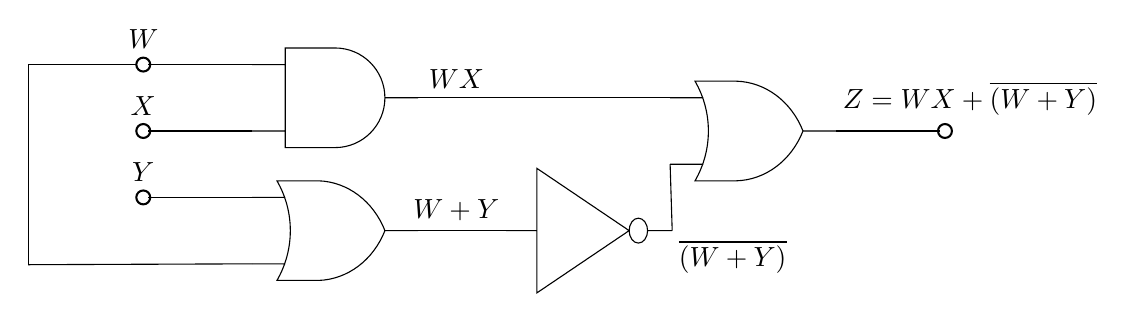
\begin{tikzpicture}[x=0.75pt,y=0.75pt,yscale=-1,xscale=1]
%uncomment if require: \path (0,393); %set diagram left start at 0, and has height of 393

%Straight Lines [id:da23815456210484298] 
\draw    (189.71,157) -- (139.64,157) ;
\draw [shift={(137.29,157)}, rotate = 180] [color={rgb, 255:red, 0; green, 0; blue, 0 }  ][line width=0.75]      (0, 0) circle [x radius= 3.35, y radius= 3.35]   ;
%Straight Lines [id:da04610179645106571] 
\draw    (189.71,189) -- (139.64,189) ;
\draw [shift={(137.29,189)}, rotate = 180] [color={rgb, 255:red, 0; green, 0; blue, 0 }  ][line width=0.75]      (0, 0) circle [x radius= 3.35, y radius= 3.35]   ;
%Shape: And Gate [id:dp1564557077664277] 
\draw   (205.71,149) -- (229.71,149) .. controls (242.96,149) and (253.71,159.75) .. (253.71,173) .. controls (253.71,186.25) and (242.96,197) .. (229.71,197) -- (205.71,197) -- (205.71,149) -- cycle (189.71,157) -- (205.71,157) (189.71,189) -- (205.71,189) (253.71,173) -- (269.71,173) ;
%Straight Lines [id:da4661863224212748] 
\draw    (391.13,173) -- (280,173) -- (269.71,173) ;
%Straight Lines [id:da6073723811431462] 
\draw    (189.71,221) -- (139.64,221) ;
\draw [shift={(137.29,221)}, rotate = 180] [color={rgb, 255:red, 0; green, 0; blue, 0 }  ][line width=0.75]      (0, 0) circle [x radius= 3.35, y radius= 3.35]   ;
%Shape: Or Gate [id:dp34982237474249467] 
\draw   (201.71,213) -- (221.71,213) .. controls (235.66,213.43) and (248.13,222.78) .. (253.71,237) .. controls (248.13,251.22) and (235.66,260.57) .. (221.71,261) -- (201.71,261) .. controls (210.29,246.15) and (210.29,227.85) .. (201.71,213) -- cycle (189.71,221) -- (205.71,221) (189.71,253) -- (205.71,253) (253.71,237) -- (269.71,237) ;
%Straight Lines [id:da4284855074469899] 
\draw    (134.29,157) -- (81.87,157) ;
%Straight Lines [id:da5958317835136014] 
\draw    (81.87,253.42) -- (81.87,157) ;
%Straight Lines [id:da993377758021355] 
\draw    (81.87,253.42) -- (189.71,253) ;
%Straight Lines [id:da05592416301039271] 
\draw    (312.13,237) -- (269.71,237) ;
%Shape: Not/Inverter Gate [id:dp7110148584625413] 
\draw   (326.95,207) -- (371.39,237) -- (326.95,267) -- (326.95,207) -- cycle (312.13,237) -- (326.95,237) (380.28,237) -- (392.13,237) (371.39,237) .. controls (371.39,233.69) and (373.38,231) .. (375.84,231) .. controls (378.29,231) and (380.28,233.69) .. (380.28,237) .. controls (380.28,240.31) and (378.29,243) .. (375.84,243) .. controls (373.38,243) and (371.39,240.31) .. (371.39,237) -- cycle ;
%Shape: Or Gate [id:dp6675241851427653] 
\draw   (403.13,165) -- (423.13,165) .. controls (437.08,165.43) and (449.55,174.78) .. (455.13,189) .. controls (449.55,203.22) and (437.08,212.57) .. (423.13,213) -- (403.13,213) .. controls (411.71,198.15) and (411.71,179.85) .. (403.13,165) -- cycle (391.13,173) -- (407.13,173) (391.13,205) -- (407.13,205) (455.13,189) -- (471.13,189) ;
%Straight Lines [id:da5356554710077354] 
\draw    (392.13,237) -- (391.13,205) ;
%Straight Lines [id:da3264629812941331] 
\draw    (471.13,189) -- (521.2,189) ;
\draw [shift={(523.55,189)}, rotate = 0] [color={rgb, 255:red, 0; green, 0; blue, 0 }  ][line width=0.75]      (0, 0) circle [x radius= 3.35, y radius= 3.35]   ;

% Text Node
\draw (137.29,150.6) node [anchor=south] [inner sep=0.75pt]    {$W$};
% Text Node
\draw (137.29,182.6) node [anchor=south] [inner sep=0.75pt]    {$X$};
% Text Node
\draw (288.13,169.6) node [anchor=south] [inner sep=0.75pt]    {$WX$};
% Text Node
\draw (137.29,214.6) node [anchor=south] [inner sep=0.75pt]    {$Y$};
% Text Node
\draw (288.13,233.6) node [anchor=south] [inner sep=0.75pt]    {$W+Y$};
% Text Node
\draw (394.13,240.4) node [anchor=north west][inner sep=0.75pt]    {$\overline{( W+Y)}$};
% Text Node
\draw (473.13,182.6) node [anchor=south west] [inner sep=0.75pt]    {$Z=WX+\overline{( W+Y)}$};


\end{tikzpicture}

          \caption{Logic Circuit for 1c}
          \label{fig:3}
        \end{figure}

    \end{enumerate}

  \item We can calculate the noise margins as:

    $$NM_H=V_{OH}-V_{IH}$$
    $$NM_L=V_{IL}-V_{OL}$$

    This gives us:

    $$NM_H=4.5-3$$
    $$NM_L=1.5-1$$

    And finally:

    $$\boxed{NM_L=.5[\si{\volt}]\quad\text{ and }\quad NM_H=1.5[\si{\volt}]}$$

  \item The switching times may be calculated using:

    $$t_{PHL}=\frac{C_LV_{DD}}{\left( \frac{W}{L} \right)_nKP_n(V_{DD}-V_{ton})^2}$$

    \begin{center}
      and
    \end{center}

    $$t_{PLH}=\frac{C_LV_{DD}}{\left( \frac{W}{L} \right)_pKP_p(V_{DD}-|V_{top}|)^2}$$

    \begin{enumerate}

      \item For $(W/L)_n=3$ and $(W/L)_p=6$, we get:

        $$t_{PHL}=\frac{(2\cdot10^{-12})(5)}{(3)(50\cdot10^{-6})(5-1)^2}$$
        $$t_{PLH}=\frac{(2\cdot10^{-12})(5)}{(6)(25\cdot10^{-6})(5-|-1|)^2}$$

        This results in:

        $$\boxed{t_{PHL}=t_{PLH}=4.166\bar{6}[\si{\nano\second}]}$$

      \item For $(W/L)_n=3$ and $(W/L)_p=60$, we get:

        $$t_{PHL}=\frac{(2\cdot10^{-12})(5)}{(3)(50\cdot10^{-6})(5-1)^2}$$
        $$t_{PLH}=\frac{(2\cdot10^{-12})(5)}{(60)(25\cdot10^{-6})(5-|-1|)^2}$$

        This results in:

        $$\boxed{t_{PHL}=4.166\bar{6}[\si{\nano\second}]\quad\text{ and }\quad t_{PLH}=.416\bar{6}[\si{\nano\second}]}$$

      \item For $(W/L)_n=30$ and $(W/L)_p=6$, we get:

        $$t_{PHL}=\frac{(2\cdot10^{-12})(5)}{(30)(50\cdot10^{-6})(5-1)^2}$$
        $$t_{PLH}=\frac{(2\cdot10^{-12})(5)}{(6)(25\cdot10^{-6})(5-|-1|)^2}$$

        This results in:

        $$\boxed{t_{PHL}=.416\bar{6}[\si{\nano\second}]\quad\text{ and }\quad t_{PLH}=4.166\bar{6}[\si{\nano\second}]}$$

    \end{enumerate}

  \item

    \begin{enumerate}

      \item Given that both transistors are expected to be in saturation, we may use our formulas to equate:

        $$I_n=\left( \frac{W}{L} \right)_n\left(\frac{KP_n}{2}\right)(V_{in}-V_{ton})^2(1+\lambda V_{DD}/2)$$
        $$I_p=\left( \frac{W}{L} \right)_p\left(\frac{KP_p}{2}\right)(V_{in}-V_{DD}-|V_{top}|)^2(1+\lambda V_{DD}/2)$$

        This allows us to rearrange and get:

        $$\frac{W_p}{W_n}=\left[ \frac{V_{in}-V_{ton}}{V_{in}-V_{DD}-|V_{top}|} \right]^2\left( \frac{KP_n}{KP_p} \right)$$

        We insert known values (and take the input as half the supply voltage) to get:

        $$\frac{W_p}{W_n}=\left[ \frac{.6-.3}{.6-1.2-|-.4|} \right]^2\left( \frac{90}{30} \right)$$

        Evaluation, we find:

        $$\boxed{\frac{W_p}{W_n}=.27}$$

      \item Taking one of our current equations from before, we get:

        $$I_n=\left( \frac{W}{L} \right)_n\left(\frac{KP_n}{2}\right)(V_{in}-V_{ton})^2(1+\lambda V_{DD}/2)$$

        We substitute the given values to get:

        $$.05\cdot10^{-3}=\left( \frac{W_n}{.12\cdot10^{-6}} \right)\left(\frac{90\cdot10^{-6}}{2}\right)(.6-.3)^2(1+.05 (.6))$$
        
        Evaluating, we find:

        $$\boxed{W_n=1.4383[\si{\micro\meter}]}$$

        Using our ratio, we obtain:

        $$W_p=.27W_n$$
        $$W_p=.27(1.4383)$$
        $$\boxed{W_p=.38835[\si{\micro\meter}]}$$

      \item The above results allow us to obtain the following DC transfer characteristics:

        \begin{figure}[H]
          \centering
          \tikzset{every picture/.style={line width=0.75pt}} %set default line width to 0.75pt        

\begin{tikzpicture}[x=0.75pt,y=0.75pt,yscale=-1,xscale=1]
%uncomment if require: \path (0,417); %set diagram left start at 0, and has height of 417

%Shape: Axis 2D [id:dp9911640907154327] 
\draw  (128,349.8) -- (479,349.8)(163.1,60) -- (163.1,382) (472,344.8) -- (479,349.8) -- (472,354.8) (158.1,67) -- (163.1,60) -- (168.1,67)  ;
%Curve Lines [id:da937920688970574] 
\draw    (164,122) .. controls (418,123) and (164,349) .. (457,346) ;
%Straight Lines [id:da3438464160916024] 
\draw [color={rgb, 255:red, 155; green, 155; blue, 155 }  ,draw opacity=1 ] [dash pattern={on 4.5pt off 4.5pt}]  (294.71,233) -- (164.29,233) ;
%Straight Lines [id:da29303419557985866] 
\draw [color={rgb, 255:red, 155; green, 155; blue, 155 }  ,draw opacity=1 ] [dash pattern={on 4.5pt off 4.5pt}]  (201.5,350.21) -- (201.5,123.79) ;
%Straight Lines [id:da5755342108389278] 
\draw [color={rgb, 255:red, 155; green, 155; blue, 155 }  ,draw opacity=1 ] [dash pattern={on 4.5pt off 4.5pt}]  (399.5,351.21) -- (399.5,342.79) ;

% Text Node
\draw (148,39.4) node [anchor=north west][inner sep=0.75pt]    {$V_{out}$};
% Text Node
\draw (481,349.4) node [anchor=north west][inner sep=0.75pt]    {$V_{in}$};
% Text Node
\draw (162,122) node [anchor=east] [inner sep=0.75pt]    {$1.2[ V]$};
% Text Node
\draw (162.29,233) node [anchor=east] [inner sep=0.75pt]    {$.6[ V]$};
% Text Node
\draw (161.1,353.2) node [anchor=north east] [inner sep=0.75pt]    {$0$};
% Text Node
\draw (201.5,353.61) node [anchor=north] [inner sep=0.75pt]    {$V_{ton}$};
% Text Node
\draw (399.5,354.61) node [anchor=north] [inner sep=0.75pt]    {$1.2-V_{top}$};
% Text Node
\draw (296.71,229.6) node [anchor=south west] [inner sep=0.75pt]    {$\frac{V_{DD}}{2}$};


\end{tikzpicture}

          \caption{DC Transfer Characteristics of CMOS Inverter}
          \label{fig:4}
        \end{figure}

    \end{enumerate}

  \item Power dissipation of a CMOS is given by:

    $$P_d=CfV_{DD}^2$$

    Substituting our known values gives us:

    $$P_d=(100\cdot10^{-15})(100\cdot10^6)(3)^2$$

    Thus we get:

    $$\boxed{P_d=9\cdot10^{-5}[\si{\watt}]}$$

    Note that there is no dissipation when $V_{DD}=0[\si{\volt}]$

  \item The pull-up network may be drawn as:

    \begin{figure}[H]
      \centering
      \tikzset{every picture/.style={line width=0.75pt}} %set default line width to 0.75pt        

\begin{tikzpicture}[x=0.75pt,y=0.75pt,yscale=-1,xscale=1]
%uncomment if require: \path (0,393); %set diagram left start at 0, and has height of 393

%Straight Lines [id:da45501350029602516] 
\draw    (89.36,135) -- (65.29,135) ;
\draw [shift={(65.29,135)}, rotate = 180] [color={rgb, 255:red, 0; green, 0; blue, 0 }  ][fill={rgb, 255:red, 0; green, 0; blue, 0 }  ][line width=0.75]      (0, 0) circle [x radius= 3.35, y radius= 3.35]   ;
\draw [shift={(91.71,135)}, rotate = 180] [color={rgb, 255:red, 0; green, 0; blue, 0 }  ][line width=0.75]      (0, 0) circle [x radius= 3.35, y radius= 3.35]   ;
%Straight Lines [id:da9060964154428524] 
\draw    (95.71,123.79) -- (95.71,146.21) ;
%Straight Lines [id:da8086629056678378] 
\draw    (101.71,123.79) -- (101.71,146.21) ;
%Straight Lines [id:da25756473565471727] 
\draw    (124.13,123.79) -- (101.71,123.79) ;
%Straight Lines [id:da31496297391065653] 
\draw    (124.13,146.21) -- (101.71,146.21) ;
%Straight Lines [id:da7102869079070778] 
\draw    (124.13,101.37) -- (124.13,123.79) ;
%Straight Lines [id:da31912587936909254] 
\draw    (124.13,146.21) -- (124.13,168.63) ;

%Straight Lines [id:da8939458575446572] 
\draw    (237.06,102) -- (261.13,102) ;
\draw [shift={(261.13,102)}, rotate = 0] [color={rgb, 255:red, 0; green, 0; blue, 0 }  ][fill={rgb, 255:red, 0; green, 0; blue, 0 }  ][line width=0.75]      (0, 0) circle [x radius= 3.35, y radius= 3.35]   ;
\draw [shift={(234.71,102)}, rotate = 0] [color={rgb, 255:red, 0; green, 0; blue, 0 }  ][line width=0.75]      (0, 0) circle [x radius= 3.35, y radius= 3.35]   ;
%Straight Lines [id:da1593078230789633] 
\draw    (230.71,113.21) -- (230.71,90.79) ;
%Straight Lines [id:da6437527822660468] 
\draw    (224.71,113.21) -- (224.71,90.79) ;
%Straight Lines [id:da3836120051079601] 
\draw    (202.29,113.21) -- (224.71,113.21) ;
%Straight Lines [id:da9974466767401046] 
\draw    (202.29,90.79) -- (224.71,90.79) ;
%Straight Lines [id:da8572656002282943] 
\draw    (202.29,135.63) -- (202.29,113.21) ;
%Straight Lines [id:da2011611966684762] 
\draw    (202.29,90.79) -- (202.29,68.37) ;

%Straight Lines [id:da9685790223986392] 
\draw    (237.06,167) -- (261.13,167) ;
\draw [shift={(261.13,167)}, rotate = 0] [color={rgb, 255:red, 0; green, 0; blue, 0 }  ][fill={rgb, 255:red, 0; green, 0; blue, 0 }  ][line width=0.75]      (0, 0) circle [x radius= 3.35, y radius= 3.35]   ;
\draw [shift={(234.71,167)}, rotate = 0] [color={rgb, 255:red, 0; green, 0; blue, 0 }  ][line width=0.75]      (0, 0) circle [x radius= 3.35, y radius= 3.35]   ;
%Straight Lines [id:da7372870285143324] 
\draw    (230.71,178.21) -- (230.71,155.79) ;
%Straight Lines [id:da5599614279412598] 
\draw    (224.71,178.21) -- (224.71,155.79) ;
%Straight Lines [id:da7099645196476283] 
\draw    (202.29,178.21) -- (224.71,178.21) ;
%Straight Lines [id:da0672451783756467] 
\draw    (202.29,155.79) -- (224.71,155.79) ;
%Straight Lines [id:da43074855563878534] 
\draw    (202.29,200.63) -- (202.29,178.21) ;
%Straight Lines [id:da7929790111436603] 
\draw    (202.29,155.79) -- (202.29,133.37) ;

%Straight Lines [id:da7037001509318173] 
\draw    (124.13,67.74) -- (202.29,68.37) ;
%Straight Lines [id:da949953903411853] 
\draw    (124.13,67.74) -- (124.13,101.37) ;
%Straight Lines [id:da7992704578689389] 
\draw    (124.13,168.63) -- (124.13,200) ;
%Straight Lines [id:da07589502430216877] 
\draw    (124.13,200) -- (202.29,200.63) ;
%Straight Lines [id:da9180363691872458] 
\draw [line width=1.5]    (163.21,68.05) -- (163.21,30.63) ;
\draw [shift={(163.21,27.63)}, rotate = 90] [color={rgb, 255:red, 0; green, 0; blue, 0 }  ][line width=1.5]    (14.21,-4.28) .. controls (9.04,-1.82) and (4.3,-0.39) .. (0,0) .. controls (4.3,0.39) and (9.04,1.82) .. (14.21,4.28)   ;
%Straight Lines [id:da26038617273148923] 
\draw    (163.21,200.32) -- (163.21,231.68) ;
%Straight Lines [id:da245887074299888] 
\draw    (89.36,265) -- (65.29,265) ;
\draw [shift={(65.29,265)}, rotate = 180] [color={rgb, 255:red, 0; green, 0; blue, 0 }  ][fill={rgb, 255:red, 0; green, 0; blue, 0 }  ][line width=0.75]      (0, 0) circle [x radius= 3.35, y radius= 3.35]   ;
\draw [shift={(91.71,265)}, rotate = 180] [color={rgb, 255:red, 0; green, 0; blue, 0 }  ][line width=0.75]      (0, 0) circle [x radius= 3.35, y radius= 3.35]   ;
%Straight Lines [id:da654593798160285] 
\draw    (95.71,253.79) -- (95.71,276.21) ;
%Straight Lines [id:da7020142501061837] 
\draw    (101.71,253.79) -- (101.71,276.21) ;
%Straight Lines [id:da7619774699922724] 
\draw    (124.13,253.79) -- (101.71,253.79) ;
%Straight Lines [id:da21793501758531497] 
\draw    (124.13,276.21) -- (101.71,276.21) ;
%Straight Lines [id:da7543333463145466] 
\draw    (124.13,231.37) -- (124.13,253.79) ;
%Straight Lines [id:da10751316879527639] 
\draw    (124.13,276.21) -- (124.13,298.63) ;

%Straight Lines [id:da9090942274028935] 
\draw    (124.13,231.37) -- (202.29,232) ;
%Straight Lines [id:da024700879185209024] 
\draw    (236.06,266) -- (260.13,266) ;
\draw [shift={(260.13,266)}, rotate = 0] [color={rgb, 255:red, 0; green, 0; blue, 0 }  ][fill={rgb, 255:red, 0; green, 0; blue, 0 }  ][line width=0.75]      (0, 0) circle [x radius= 3.35, y radius= 3.35]   ;
\draw [shift={(233.71,266)}, rotate = 0] [color={rgb, 255:red, 0; green, 0; blue, 0 }  ][line width=0.75]      (0, 0) circle [x radius= 3.35, y radius= 3.35]   ;
%Straight Lines [id:da5422078509611399] 
\draw    (229.71,277.21) -- (229.71,254.79) ;
%Straight Lines [id:da5646888646202193] 
\draw    (223.71,277.21) -- (223.71,254.79) ;
%Straight Lines [id:da914256693876994] 
\draw    (201.29,277.21) -- (223.71,277.21) ;
%Straight Lines [id:da8214819062960135] 
\draw    (201.29,254.79) -- (223.71,254.79) ;
%Straight Lines [id:da9245687681073022] 
\draw    (201.29,299.63) -- (201.29,277.21) ;
%Straight Lines [id:da27729352765401705] 
\draw    (201.29,254.79) -- (201.29,232.37) ;

%Straight Lines [id:da45809668968788764] 
\draw    (123.13,299) -- (201.29,299.63) ;

% Text Node
\draw (163.21,24.23) node [anchor=south] [inner sep=0.75pt]    {$V_{CC}$};
% Text Node
\draw (61.29,135) node [anchor=east] [inner sep=0.75pt]    {$A$};
% Text Node
\draw (61.29,265) node [anchor=east] [inner sep=0.75pt]    {$D$};
% Text Node
\draw (265.13,102) node [anchor=west] [inner sep=0.75pt]    {$B$};
% Text Node
\draw (265.13,167) node [anchor=west] [inner sep=0.75pt]    {$C$};
% Text Node
\draw (264.13,266) node [anchor=west] [inner sep=0.75pt]    {$E$};


\end{tikzpicture}

      \caption{Corresponding Pull-Up Network}
      \label{fig:5}
    \end{figure}

    The pull-down network then becomes:

    \begin{figure}[H]
      \centering
      \tikzset{every picture/.style={line width=0.75pt}} %set default line width to 0.75pt        

\begin{tikzpicture}[x=0.75pt,y=0.75pt,yscale=-1,xscale=1]
%uncomment if require: \path (0,393); %set diagram left start at 0, and has height of 393

%Straight Lines [id:da6669314469470796] 
\draw    (533.71,124) -- (565.13,124) ;
\draw [shift={(565.13,124)}, rotate = 0] [color={rgb, 255:red, 0; green, 0; blue, 0 }  ][fill={rgb, 255:red, 0; green, 0; blue, 0 }  ][line width=0.75]      (0, 0) circle [x radius= 3.35, y radius= 3.35]   ;
%Straight Lines [id:da6639068051977447] 
\draw    (534.71,135.21) -- (534.71,112.79) ;
%Straight Lines [id:da8531260057533494] 
\draw    (528.71,135.21) -- (528.71,112.79) ;
%Straight Lines [id:da11917849895029109] 
\draw    (506.29,135.21) -- (528.71,135.21) ;
%Straight Lines [id:da8885698531337861] 
\draw    (506.29,112.79) -- (528.71,112.79) ;
%Straight Lines [id:da47029761972586415] 
\draw    (506.29,157.63) -- (506.29,135.21) ;
%Straight Lines [id:da3420382268981802] 
\draw    (506.29,112.79) -- (506.29,90.37) ;

%Straight Lines [id:da8454011253884546] 
\draw    (572.71,191) -- (604.13,191) ;
\draw [shift={(604.13,191)}, rotate = 0] [color={rgb, 255:red, 0; green, 0; blue, 0 }  ][fill={rgb, 255:red, 0; green, 0; blue, 0 }  ][line width=0.75]      (0, 0) circle [x radius= 3.35, y radius= 3.35]   ;
%Straight Lines [id:da28991151339977816] 
\draw    (573.71,202.21) -- (573.71,179.79) ;
%Straight Lines [id:da11726155815340011] 
\draw    (567.71,202.21) -- (567.71,179.79) ;
%Straight Lines [id:da999923146603045] 
\draw    (545.29,202.21) -- (567.71,202.21) ;
%Straight Lines [id:da6411228717849907] 
\draw    (545.29,179.79) -- (567.71,179.79) ;
%Straight Lines [id:da32550941533121147] 
\draw    (545.29,224.63) -- (545.29,202.21) ;
%Straight Lines [id:da14385413534039093] 
\draw    (545.29,179.79) -- (545.29,157.37) ;

%Straight Lines [id:da7748188250025749] 
\draw    (467.21,157.32) -- (545.37,157.95) ;
%Straight Lines [id:da455000338079496] 
\draw    (439.71,191) -- (408.29,191) ;
\draw [shift={(408.29,191)}, rotate = 180] [color={rgb, 255:red, 0; green, 0; blue, 0 }  ][fill={rgb, 255:red, 0; green, 0; blue, 0 }  ][line width=0.75]      (0, 0) circle [x radius= 3.35, y radius= 3.35]   ;
%Straight Lines [id:da46816519455905425] 
\draw    (438.71,179.79) -- (438.71,202.21) ;
%Straight Lines [id:da6215796318599741] 
\draw    (444.71,179.79) -- (444.71,202.21) ;
%Straight Lines [id:da3766903464517315] 
\draw    (467.13,179.79) -- (444.71,179.79) ;
%Straight Lines [id:da6283797118249942] 
\draw    (467.13,202.21) -- (444.71,202.21) ;
%Straight Lines [id:da8583756635913542] 
\draw    (467.13,157.37) -- (467.13,179.79) ;
%Straight Lines [id:da2959109136231264] 
\draw    (467.13,202.21) -- (467.13,224.63) ;

%Straight Lines [id:da4538599972513643] 
\draw    (467.13,224) -- (545.29,224.63) ;
%Straight Lines [id:da008192227675895891] 
\draw    (349.97,89.1) -- (506.29,90.37) ;
%Straight Lines [id:da33588774461519344] 
\draw    (322.71,123) -- (291.29,123) ;
\draw [shift={(291.29,123)}, rotate = 180] [color={rgb, 255:red, 0; green, 0; blue, 0 }  ][fill={rgb, 255:red, 0; green, 0; blue, 0 }  ][line width=0.75]      (0, 0) circle [x radius= 3.35, y radius= 3.35]   ;
%Straight Lines [id:da2603844285428878] 
\draw    (321.71,111.79) -- (321.71,134.21) ;
%Straight Lines [id:da3047784086308962] 
\draw    (327.71,111.79) -- (327.71,134.21) ;
%Straight Lines [id:da579368725340582] 
\draw    (350.13,111.79) -- (327.71,111.79) ;
%Straight Lines [id:da9482423215739264] 
\draw    (350.13,134.21) -- (327.71,134.21) ;
%Straight Lines [id:da25077744492411924] 
\draw    (350.13,89.37) -- (350.13,111.79) ;
%Straight Lines [id:da18269772712684895] 
\draw    (350.13,134.21) -- (350.13,156.63) ;

%Straight Lines [id:da46594156620486904] 
\draw    (322.71,189) -- (291.29,189) ;
\draw [shift={(291.29,189)}, rotate = 180] [color={rgb, 255:red, 0; green, 0; blue, 0 }  ][fill={rgb, 255:red, 0; green, 0; blue, 0 }  ][line width=0.75]      (0, 0) circle [x radius= 3.35, y radius= 3.35]   ;
%Straight Lines [id:da5491180035921359] 
\draw    (321.71,177.79) -- (321.71,200.21) ;
%Straight Lines [id:da7434221443738968] 
\draw    (327.71,177.79) -- (327.71,200.21) ;
%Straight Lines [id:da9819688427768148] 
\draw    (350.13,177.79) -- (327.71,177.79) ;
%Straight Lines [id:da3022480303057826] 
\draw    (350.13,200.21) -- (327.71,200.21) ;
%Straight Lines [id:da01815089079461263] 
\draw    (350.13,155.37) -- (350.13,177.79) ;
%Straight Lines [id:da4605867555621066] 
\draw    (350.13,200.21) -- (350.13,222.63) ;

%Straight Lines [id:da8823471900240443] 
\draw    (350.13,222.63) -- (350.13,254) ;
%Straight Lines [id:da8058062951400016] 
\draw    (506.21,224.32) -- (506.21,255.68) ;
%Straight Lines [id:da8657784198277411] 
\draw    (350.13,254) -- (506.21,255.68) ;
%Straight Lines [id:da11573673398382955] 
\draw    (428.17,254.84) -- (428.17,286.21) ;
%Straight Lines [id:da3970811655856984] 
\draw    (443.86,290.21) -- (412.49,290.21) ;
%Straight Lines [id:da7336048867351443] 
\draw    (440.86,294.21) -- (415.49,294.21) ;
%Straight Lines [id:da41031232767902925] 
\draw    (437.86,298.21) -- (418.49,298.21) ;

% Text Node
\draw (569.13,124) node [anchor=west] [inner sep=0.75pt]    {$A$};
% Text Node
\draw (608.13,191) node [anchor=west] [inner sep=0.75pt]    {$C$};
% Text Node
\draw (403.29,191) node [anchor=east] [inner sep=0.75pt]    {$B$};
% Text Node
\draw (287.29,123) node [anchor=east] [inner sep=0.75pt]    {$D$};
% Text Node
\draw (287.29,189) node [anchor=east] [inner sep=0.75pt]    {$E$};


\end{tikzpicture}

      \caption{Corresponding Pull-Down Network}
      \label{fig:6}
    \end{figure}

    We combine the two to form the full network:

    \begin{figure}[H]
      \centering
      \tikzset{every picture/.style={line width=0.75pt}} %set default line width to 0.75pt        

\begin{tikzpicture}[x=0.75pt,y=0.75pt,yscale=-.8,xscale=.8]
%uncomment if require: \path (0,593); %set diagram left start at 0, and has height of 593

%Straight Lines [id:da45501350029602516] 
\draw    (89.36,135) -- (65.29,135) ;
\draw [shift={(65.29,135)}, rotate = 180] [color={rgb, 255:red, 0; green, 0; blue, 0 }  ][fill={rgb, 255:red, 0; green, 0; blue, 0 }  ][line width=0.75]      (0, 0) circle [x radius= 3.35, y radius= 3.35]   ;
\draw [shift={(91.71,135)}, rotate = 180] [color={rgb, 255:red, 0; green, 0; blue, 0 }  ][line width=0.75]      (0, 0) circle [x radius= 3.35, y radius= 3.35]   ;
%Straight Lines [id:da9060964154428524] 
\draw    (95.71,123.79) -- (95.71,146.21) ;
%Straight Lines [id:da8086629056678378] 
\draw    (101.71,123.79) -- (101.71,146.21) ;
%Straight Lines [id:da25756473565471727] 
\draw    (124.13,123.79) -- (101.71,123.79) ;
%Straight Lines [id:da31496297391065653] 
\draw    (124.13,146.21) -- (101.71,146.21) ;
%Straight Lines [id:da7102869079070778] 
\draw    (124.13,101.37) -- (124.13,123.79) ;
%Straight Lines [id:da31912587936909254] 
\draw    (124.13,146.21) -- (124.13,168.63) ;

%Straight Lines [id:da8939458575446572] 
\draw    (237.06,102) -- (261.13,102) ;
\draw [shift={(261.13,102)}, rotate = 0] [color={rgb, 255:red, 0; green, 0; blue, 0 }  ][fill={rgb, 255:red, 0; green, 0; blue, 0 }  ][line width=0.75]      (0, 0) circle [x radius= 3.35, y radius= 3.35]   ;
\draw [shift={(234.71,102)}, rotate = 0] [color={rgb, 255:red, 0; green, 0; blue, 0 }  ][line width=0.75]      (0, 0) circle [x radius= 3.35, y radius= 3.35]   ;
%Straight Lines [id:da1593078230789633] 
\draw    (230.71,113.21) -- (230.71,90.79) ;
%Straight Lines [id:da6437527822660468] 
\draw    (224.71,113.21) -- (224.71,90.79) ;
%Straight Lines [id:da3836120051079601] 
\draw    (202.29,113.21) -- (224.71,113.21) ;
%Straight Lines [id:da9974466767401046] 
\draw    (202.29,90.79) -- (224.71,90.79) ;
%Straight Lines [id:da8572656002282943] 
\draw    (202.29,135.63) -- (202.29,113.21) ;
%Straight Lines [id:da2011611966684762] 
\draw    (202.29,90.79) -- (202.29,68.37) ;

%Straight Lines [id:da9685790223986392] 
\draw    (237.06,167) -- (261.13,167) ;
\draw [shift={(261.13,167)}, rotate = 0] [color={rgb, 255:red, 0; green, 0; blue, 0 }  ][fill={rgb, 255:red, 0; green, 0; blue, 0 }  ][line width=0.75]      (0, 0) circle [x radius= 3.35, y radius= 3.35]   ;
\draw [shift={(234.71,167)}, rotate = 0] [color={rgb, 255:red, 0; green, 0; blue, 0 }  ][line width=0.75]      (0, 0) circle [x radius= 3.35, y radius= 3.35]   ;
%Straight Lines [id:da7372870285143324] 
\draw    (230.71,178.21) -- (230.71,155.79) ;
%Straight Lines [id:da5599614279412598] 
\draw    (224.71,178.21) -- (224.71,155.79) ;
%Straight Lines [id:da7099645196476283] 
\draw    (202.29,178.21) -- (224.71,178.21) ;
%Straight Lines [id:da0672451783756467] 
\draw    (202.29,155.79) -- (224.71,155.79) ;
%Straight Lines [id:da43074855563878534] 
\draw    (202.29,200.63) -- (202.29,178.21) ;
%Straight Lines [id:da7929790111436603] 
\draw    (202.29,155.79) -- (202.29,133.37) ;

%Straight Lines [id:da7037001509318173] 
\draw    (124.13,67.74) -- (202.29,68.37) ;
%Straight Lines [id:da949953903411853] 
\draw    (124.13,67.74) -- (124.13,101.37) ;
%Straight Lines [id:da7992704578689389] 
\draw    (124.13,168.63) -- (124.13,200) ;
%Straight Lines [id:da07589502430216877] 
\draw    (124.13,200) -- (202.29,200.63) ;
%Straight Lines [id:da9180363691872458] 
\draw [line width=1.5]    (163.21,68.05) -- (163.21,30.63) ;
\draw [shift={(163.21,27.63)}, rotate = 90] [color={rgb, 255:red, 0; green, 0; blue, 0 }  ][line width=1.5]    (14.21,-4.28) .. controls (9.04,-1.82) and (4.3,-0.39) .. (0,0) .. controls (4.3,0.39) and (9.04,1.82) .. (14.21,4.28)   ;
%Straight Lines [id:da26038617273148923] 
\draw    (163.21,200.32) -- (163.21,231.68) ;
%Straight Lines [id:da245887074299888] 
\draw    (89.36,265) -- (65.29,265) ;
\draw [shift={(65.29,265)}, rotate = 180] [color={rgb, 255:red, 0; green, 0; blue, 0 }  ][fill={rgb, 255:red, 0; green, 0; blue, 0 }  ][line width=0.75]      (0, 0) circle [x radius= 3.35, y radius= 3.35]   ;
\draw [shift={(91.71,265)}, rotate = 180] [color={rgb, 255:red, 0; green, 0; blue, 0 }  ][line width=0.75]      (0, 0) circle [x radius= 3.35, y radius= 3.35]   ;
%Straight Lines [id:da654593798160285] 
\draw    (95.71,253.79) -- (95.71,276.21) ;
%Straight Lines [id:da7020142501061837] 
\draw    (101.71,253.79) -- (101.71,276.21) ;
%Straight Lines [id:da7619774699922724] 
\draw    (124.13,253.79) -- (101.71,253.79) ;
%Straight Lines [id:da21793501758531497] 
\draw    (124.13,276.21) -- (101.71,276.21) ;
%Straight Lines [id:da7543333463145466] 
\draw    (124.13,231.37) -- (124.13,253.79) ;
%Straight Lines [id:da10751316879527639] 
\draw    (124.13,276.21) -- (124.13,298.63) ;

%Straight Lines [id:da9090942274028935] 
\draw    (124.13,231.37) -- (202.29,232) ;
%Straight Lines [id:da024700879185209024] 
\draw    (236.06,266) -- (260.13,266) ;
\draw [shift={(260.13,266)}, rotate = 0] [color={rgb, 255:red, 0; green, 0; blue, 0 }  ][fill={rgb, 255:red, 0; green, 0; blue, 0 }  ][line width=0.75]      (0, 0) circle [x radius= 3.35, y radius= 3.35]   ;
\draw [shift={(233.71,266)}, rotate = 0] [color={rgb, 255:red, 0; green, 0; blue, 0 }  ][line width=0.75]      (0, 0) circle [x radius= 3.35, y radius= 3.35]   ;
%Straight Lines [id:da5422078509611399] 
\draw    (229.71,277.21) -- (229.71,254.79) ;
%Straight Lines [id:da5646888646202193] 
\draw    (223.71,277.21) -- (223.71,254.79) ;
%Straight Lines [id:da914256693876994] 
\draw    (201.29,277.21) -- (223.71,277.21) ;
%Straight Lines [id:da8214819062960135] 
\draw    (201.29,254.79) -- (223.71,254.79) ;
%Straight Lines [id:da9245687681073022] 
\draw    (201.29,299.63) -- (201.29,277.21) ;
%Straight Lines [id:da27729352765401705] 
\draw    (201.29,254.79) -- (201.29,232.37) ;

%Straight Lines [id:da45809668968788764] 
\draw    (123.13,299) -- (201.29,299.63) ;
%Straight Lines [id:da6669314469470796] 
\draw    (268.71,365) -- (300.13,365) ;
\draw [shift={(300.13,365)}, rotate = 0] [color={rgb, 255:red, 0; green, 0; blue, 0 }  ][fill={rgb, 255:red, 0; green, 0; blue, 0 }  ][line width=0.75]      (0, 0) circle [x radius= 3.35, y radius= 3.35]   ;
%Straight Lines [id:da6639068051977447] 
\draw    (269.71,376.21) -- (269.71,353.79) ;
%Straight Lines [id:da8531260057533494] 
\draw    (263.71,376.21) -- (263.71,353.79) ;
%Straight Lines [id:da11917849895029109] 
\draw    (241.29,376.21) -- (263.71,376.21) ;
%Straight Lines [id:da8885698531337861] 
\draw    (241.29,353.79) -- (263.71,353.79) ;
%Straight Lines [id:da47029761972586415] 
\draw    (241.29,398.63) -- (241.29,376.21) ;
%Straight Lines [id:da3420382268981802] 
\draw    (241.29,353.79) -- (241.29,331.37) ;

%Straight Lines [id:da8454011253884546] 
\draw    (307.71,432) -- (339.13,432) ;
\draw [shift={(339.13,432)}, rotate = 0] [color={rgb, 255:red, 0; green, 0; blue, 0 }  ][fill={rgb, 255:red, 0; green, 0; blue, 0 }  ][line width=0.75]      (0, 0) circle [x radius= 3.35, y radius= 3.35]   ;
%Straight Lines [id:da28991151339977816] 
\draw    (308.71,443.21) -- (308.71,420.79) ;
%Straight Lines [id:da11726155815340011] 
\draw    (302.71,443.21) -- (302.71,420.79) ;
%Straight Lines [id:da999923146603045] 
\draw    (280.29,443.21) -- (302.71,443.21) ;
%Straight Lines [id:da6411228717849907] 
\draw    (280.29,420.79) -- (302.71,420.79) ;
%Straight Lines [id:da32550941533121147] 
\draw    (280.29,465.63) -- (280.29,443.21) ;
%Straight Lines [id:da14385413534039093] 
\draw    (280.29,420.79) -- (280.29,398.37) ;

%Straight Lines [id:da7748188250025749] 
\draw    (202.21,398.32) -- (280.37,398.95) ;
%Straight Lines [id:da455000338079496] 
\draw    (174.71,432) -- (143.29,432) ;
\draw [shift={(143.29,432)}, rotate = 180] [color={rgb, 255:red, 0; green, 0; blue, 0 }  ][fill={rgb, 255:red, 0; green, 0; blue, 0 }  ][line width=0.75]      (0, 0) circle [x radius= 3.35, y radius= 3.35]   ;
%Straight Lines [id:da46816519455905425] 
\draw    (173.71,420.79) -- (173.71,443.21) ;
%Straight Lines [id:da6215796318599741] 
\draw    (179.71,420.79) -- (179.71,443.21) ;
%Straight Lines [id:da3766903464517315] 
\draw    (202.13,420.79) -- (179.71,420.79) ;
%Straight Lines [id:da6283797118249942] 
\draw    (202.13,443.21) -- (179.71,443.21) ;
%Straight Lines [id:da8583756635913542] 
\draw    (202.13,398.37) -- (202.13,420.79) ;
%Straight Lines [id:da2959109136231264] 
\draw    (202.13,443.21) -- (202.13,465.63) ;

%Straight Lines [id:da4538599972513643] 
\draw    (202.13,465) -- (280.29,465.63) ;
%Straight Lines [id:da008192227675895891] 
\draw    (84.97,330.1) -- (241.29,331.37) ;
%Straight Lines [id:da33588774461519344] 
\draw    (57.71,364) -- (26.29,364) ;
\draw [shift={(26.29,364)}, rotate = 180] [color={rgb, 255:red, 0; green, 0; blue, 0 }  ][fill={rgb, 255:red, 0; green, 0; blue, 0 }  ][line width=0.75]      (0, 0) circle [x radius= 3.35, y radius= 3.35]   ;
%Straight Lines [id:da2603844285428878] 
\draw    (56.71,352.79) -- (56.71,375.21) ;
%Straight Lines [id:da3047784086308962] 
\draw    (62.71,352.79) -- (62.71,375.21) ;
%Straight Lines [id:da579368725340582] 
\draw    (85.13,352.79) -- (62.71,352.79) ;
%Straight Lines [id:da9482423215739264] 
\draw    (85.13,375.21) -- (62.71,375.21) ;
%Straight Lines [id:da25077744492411924] 
\draw    (85.13,330.37) -- (85.13,352.79) ;
%Straight Lines [id:da18269772712684895] 
\draw    (85.13,375.21) -- (85.13,397.63) ;

%Straight Lines [id:da46594156620486904] 
\draw    (57.71,430) -- (26.29,430) ;
\draw [shift={(26.29,430)}, rotate = 180] [color={rgb, 255:red, 0; green, 0; blue, 0 }  ][fill={rgb, 255:red, 0; green, 0; blue, 0 }  ][line width=0.75]      (0, 0) circle [x radius= 3.35, y radius= 3.35]   ;
%Straight Lines [id:da5491180035921359] 
\draw    (56.71,418.79) -- (56.71,441.21) ;
%Straight Lines [id:da7434221443738968] 
\draw    (62.71,418.79) -- (62.71,441.21) ;
%Straight Lines [id:da9819688427768148] 
\draw    (85.13,418.79) -- (62.71,418.79) ;
%Straight Lines [id:da3022480303057826] 
\draw    (85.13,441.21) -- (62.71,441.21) ;
%Straight Lines [id:da01815089079461263] 
\draw    (85.13,396.37) -- (85.13,418.79) ;
%Straight Lines [id:da4605867555621066] 
\draw    (85.13,441.21) -- (85.13,463.63) ;

%Straight Lines [id:da8823471900240443] 
\draw    (85.13,463.63) -- (85.13,495) ;
%Straight Lines [id:da8058062951400016] 
\draw    (241.21,465.32) -- (241.21,496.68) ;
%Straight Lines [id:da8657784198277411] 
\draw    (85.13,495) -- (241.21,496.68) ;
%Straight Lines [id:da11573673398382955] 
\draw    (163.17,495.84) -- (163.17,527.21) ;
%Straight Lines [id:da3970811655856984] 
\draw    (178.86,531.21) -- (147.49,531.21) ;
%Straight Lines [id:da7336048867351443] 
\draw    (175.86,535.21) -- (150.49,535.21) ;
%Straight Lines [id:da41031232767902925] 
\draw    (172.86,539.21) -- (153.49,539.21) ;
%Straight Lines [id:da5508627759023181] 
\draw    (162.21,299.32) -- (162.21,330.68) ;
%Straight Lines [id:da9127811141529196] 
\draw    (162.21,315) -- (318.53,316.26) ;
\draw [shift={(318.53,316.26)}, rotate = 0.46] [color={rgb, 255:red, 0; green, 0; blue, 0 }  ][fill={rgb, 255:red, 0; green, 0; blue, 0 }  ][line width=0.75]      (0, 0) circle [x radius= 3.35, y radius= 3.35]   ;

% Text Node
\draw (163.21,24.23) node [anchor=south] [inner sep=0.75pt]    {$V_{CC}$};
% Text Node
\draw (61.29,135) node [anchor=east] [inner sep=0.75pt]    {$A$};
% Text Node
\draw (61.29,265) node [anchor=east] [inner sep=0.75pt]    {$D$};
% Text Node
\draw (265.13,102) node [anchor=west] [inner sep=0.75pt]    {$B$};
% Text Node
\draw (265.13,167) node [anchor=west] [inner sep=0.75pt]    {$C$};
% Text Node
\draw (264.13,266) node [anchor=west] [inner sep=0.75pt]    {$E$};
% Text Node
\draw (304.13,365) node [anchor=west] [inner sep=0.75pt]    {$A$};
% Text Node
\draw (343.13,432) node [anchor=west] [inner sep=0.75pt]    {$C$};
% Text Node
\draw (138.29,432) node [anchor=east] [inner sep=0.75pt]    {$B$};
% Text Node
\draw (22.29,364) node [anchor=east] [inner sep=0.75pt]    {$D$};
% Text Node
\draw (22.29,430) node [anchor=east] [inner sep=0.75pt]    {$E$};
% Text Node
\draw (322.53,316.26) node [anchor=west] [inner sep=0.75pt]    {$Y$};


\end{tikzpicture}

      \caption{Corresponding Network}
      \label{fig:7}
    \end{figure}

    We may observe that 10 transistors are needed, 5 for the pull-up and 5 for the pull-down networks.

  \item From the provided diagram, and a value for PMOS resistance, $R_p$, we may observe:

    $$R_{M1}=R_p\quad\text{ and }R_{M2}+R_{M3}=R_p$$

    Furthermore, since we are using the same PMOS transistors, we may write:

    $$R_{M2}=R_{M3}\Longrightarrow 2R_{M2}=2R_{M3}=R_p$$

    This means that:

    $$\boxed{\left( \frac{W}{L} \right)_{M1}=\left( \frac{W}{L} \right)_{p}}$$
    $$\boxed{\left( \frac{W}{L} \right)_{M2}=\left( \frac{W}{L} \right)_{M3}=2\left( \frac{W}{L} \right)_{p}}$$

    We can see that, for the pull-down branch, we have:

    $$R_{M4}+R_{M5}=R_n\quad\text{ and }R_{M4}=R_{M5}$$

    This gets us:

    $$\boxed{\left( \frac{W}{L} \right)_{M4}=\left( \frac{W}{L} \right)_{M5}=2\left( \frac{W}{L} \right)_{n}}$$

    We can see that the sixth transistor is equivalent to this, and we get our last value as:

    $$\boxed{\left( \frac{W}{L} \right)_{M6}=2\left( \frac{W}{L} \right)_{n}}$$

\end{enumerate}

\end{document}

